\documentclass[10pt,aspectratio=169]{beamer}

\usepackage{fontspec}
\setsansfont{Noto Sans}
\setmonofont{DejaVu Sans Mono}[Scale=0.88]
\usepackage{graphicx}
\usepackage{booktabs}
\usepackage{array}
\usepackage{tikz}
\usetikzlibrary{positioning}

\graphicspath{{shots/}}

\definecolor{ink}{HTML}{16181D}
\definecolor{mute}{HTML}{5B6270}
\definecolor{rule}{HTML}{DCDFE5}
\definecolor{paper}{HTML}{FBFAF7}
\definecolor{card}{HTML}{F1EFEA}
\definecolor{accent}{HTML}{1F5FD1}
\definecolor{patho}{HTML}{C62828}
\definecolor{warn}{HTML}{D9770F}

\setbeamercolor{background canvas}{bg=paper}
\setbeamercolor{normal text}{fg=ink}
\setbeamercolor{frametitle}{fg=ink,bg=paper}
\setbeamercolor{itemize item}{fg=accent}
\setbeamercolor{footline}{fg=mute}
\setbeamerfont{frametitle}{series=\bfseries,size=\large}
\setbeamertemplate{navigation symbols}{}
\setbeamertemplate{itemize item}{\raisebox{0.15ex}{\scriptsize$\bullet$}}
\setbeamersize{text margin left=9mm,text margin right=9mm}
\setbeamertemplate{frametitle}{%
  \vspace{5mm}%
  {\scriptsize\bfseries\color{accent}\MakeUppercase{\addfontfeature{LetterSpace=6}\insertframesubtitle}}\par
  \vspace{0.8mm}%
  {\usebeamerfont{frametitle}\insertframetitle\par}%
  \vspace{1mm}%
}
\setbeamertemplate{footline}{%
  \hspace{9mm}{\tiny Interface atlas}\hfill{\tiny\insertframenumber}\hspace{9mm}\vspace{3mm}%
}
\setlength{\leftmargini}{4mm}
\hypersetup{colorlinks,urlcolor=accent,linkcolor=ink}

\newcommand{\lede}[1]{{\small\color{mute}#1\par}\vspace{2.5mm}}
\newcommand{\shot}[3][]{%
  \begin{tikzpicture}
    \node[inner sep=0pt,draw=rule,line width=0.4pt]{\includegraphics[width=#2,clip,#1]{#3}};
  \end{tikzpicture}%
}
\newcommand{\points}[1]{\begin{itemize}\setlength{\itemsep}{2.5mm}#1\end{itemize}}
\newcommand{\smallpoints}[1]{\begin{itemize}\footnotesize\setlength{\itemsep}{1.5mm}#1\end{itemize}}
\newcommand{\headline}[1]{{\Large\bfseries\color{accent}#1}}

\usepackage{newunicodechar}
\newunicodechar{≥}{\ensuremath{\geq}}
\newunicodechar{→}{\ensuremath{\rightarrow}}

\newcommand{\orx}[1]{(#1-0.5)*9.5mm}
\newcommand{\forest}[6][accent]{%
  \node[anchor=east,font=\scriptsize] at (-2mm,#2) {#3};
  \draw[#1,line width=1pt,line cap=round] ({\orx{#5}},#2) -- ({\orx{#6}},#2);
  \fill[#1] ({\orx{#4}},#2) circle (1mm);
  \node[anchor=west,font=\scriptsize] at (37mm,#2) {\textbf{#4} {\color{mute}(#5–#6)}};
}

\begin{document}

\begin{frame}[plain]
  \vspace{6mm}
  {\scriptsize\bfseries\color{accent}\addfontfeature{LetterSpace=6}BIOHACKATHON EUROPE 2026 · PROJECT 9: FROM ALIGNMENT TO INSIGHT\par}
  \vspace{3mm}
  {\huge\bfseries Interface atlas\par}
  \vspace{4mm}
  \begin{minipage}{128mm}
    \raggedright\Large
    Proteins work by touching each other. We mapped where they touch onto the
    human genome, and disease-causing mutations pile up exactly there.
  \end{minipage}

  \vspace{8mm}
  {\small\color{mute}Try it: \url{https://cmdcolin.github.io/interface-atlas/}\\
  Progress as of 11 November 2026\par}
\end{frame}

\begin{frame}
  \frametitle{TL;DR: a mutation where two proteins touch is more likely to cause disease, and now you can look each one up}
  \framesubtitle{The whole thing on one slide}
  \vspace{1mm}
  \begin{columns}[T,onlytextwidth]
    \begin{column}{0.31\textwidth}
      {\footnotesize\bfseries\color{mute}THE IDEA\par}\vspace{1.5mm}
      \headline{handshakes}\par\vspace{1.5mm}
      {\small Most proteins do their job in pairs. Change one building block on
      the surface where they meet and the handshake can fail.\par}
    \end{column}
    \begin{column}{0.31\textwidth}
      {\footnotesize\bfseries\color{mute}WHAT WE DID\par}\vspace{1.5mm}
      \headline{5,350 proteins}\par\vspace{1.5mm}
      {\small For every human disease protein, we lined up three things: its
      contact surfaces in 3D, the DNA that codes for them, and the variants
      seen in patients.\par}
    \end{column}
    \begin{column}{0.31\textwidth}
      {\footnotesize\bfseries\color{mute}WHAT WE FOUND\par}\vspace{1.5mm}
      \headline{2.4× as often}\par\vspace{1.5mm}
      {\small Harmful variants sit on a contact surface 2.4 times as often as
      harmless ones. Another 23,233 variants that nobody can yet classify sit
      there too.\par}
    \end{column}
  \end{columns}
  \vspace{5mm}
  {\small\color{mute}The contact surfaces come from AlphaFold's predicted protein
  pairs and, for the team's receptor set, from lab-solved structures. Everything
  is on a public website with a genome browser and a 3D viewer.\par}
\end{frame}

\begin{frame}
  \frametitle{TL;DR: the project locks the 1D alignment and the 3D view together; this does the same with the genome as the 1D view}
  \framesubtitle{How it fits ``from alignment to insight''}
  \begin{columns}[T,onlytextwidth]
    \begin{column}{0.37\textwidth}
      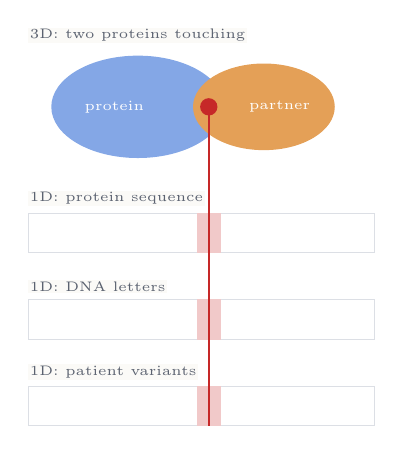
\begin{tikzpicture}[lane/.style={draw=rule,fill=white,minimum width=44mm,minimum height=5mm,inner sep=0pt,anchor=west}]
        \node[font=\tiny,anchor=south west,text=mute,inner sep=0.6pt,fill=paper] at (3mm,50mm) {3D: two proteins touching};
        \fill[accent!55] (17mm,42mm) ellipse (11mm and 6.5mm);
        \fill[warn!70] (33mm,42mm) ellipse (9mm and 5.5mm);
        \node[font=\tiny,text=white] at (14mm,42mm) {protein};
        \node[font=\tiny,text=white] at (35mm,42mm) {partner};
        \node[lane] (seq) at (3mm,26mm) {};
        \node[lane] (dna) at (3mm,15mm) {};
        \node[lane] (var) at (3mm,4mm) {};
        \foreach \l in {seq,dna,var}
          \fill[patho!25] ([xshift=21.5mm]\l.south west) rectangle ([xshift=24.5mm]\l.north west);
        \draw[patho,line width=0.9pt] (26mm,42mm) -- (26mm,1.5mm);
        \fill[patho] (26mm,42mm) circle (1.1mm);
        \node[font=\tiny,anchor=south west,text=mute,inner sep=0.6pt,fill=paper] at (3mm,29.3mm) {1D: protein sequence};
        \node[font=\tiny,anchor=south west,text=mute,inner sep=0.6pt,fill=paper] at (3mm,18.3mm) {1D: DNA letters};
        \node[font=\tiny,anchor=south west,text=mute,inner sep=0.6pt,fill=paper] at (3mm,7.3mm) {1D: patient variants};
      \end{tikzpicture}
    \end{column}
    \begin{column}{0.6\textwidth}
      {\footnotesize\renewcommand{\arraystretch}{1.5}
      \begin{tabular}{@{}>{\raggedright\arraybackslash}p{34mm}>{\raggedright\arraybackslash}p{47mm}@{}}
        \textbf{The project asks for} & \textbf{What the atlas does} \\
        \midrule
        1D and 3D locked in sync & genome browser and 3D viewer linked, side by side \\[0.8mm]
        Interaction surfaces that stand out & contact surfaces drawn as tracks for 1,331 disease genes \\[0.8mm]
        GPCRs as a demo family & the team's 45 receptor structures, G-protein contacts mapped \\[0.8mm]
        No structural expertise required & look a gene up by name, click a variant \\[0.8mm]
        Conservation on surfaces, from an alignment & not here: no multiple sequence alignment view \\[0.8mm]
      \end{tabular}}
    \end{column}
  \end{columns}
\end{frame}

\begin{frame}
  \frametitle{TL;DR: one example. A known cancer-syndrome mutation sits right where VHL grips its partner}
  \framesubtitle{What it looks like}
  \begin{columns}[T,onlytextwidth]
    \begin{column}{0.66\textwidth}
      \shot[trim=0 0 0 0]{\textwidth}{variant3d.png}
    \end{column}
    \begin{column}{0.31\textwidth}
      \points{\small
        \item \textbf{VHL} guards against tumours; inherited faults cause von
          Hippel–Lindau syndrome
        \item 27 of its 213 building blocks touch its partner;
          \textbf{48 harmful variants} sit on them
        \item Shown: one of them, S80G, on the gene (left) and in 3D (right).
          29 more on that surface are unclassified
      }
    \end{column}
  \end{columns}
\end{frame}

\begin{frame}
  \frametitle{TL;DR: harmful variants are about twice as likely to sit where proteins touch}
  \framesubtitle{The main result}
  \begin{columns}[T,onlytextwidth]
    \begin{column}{0.55\textwidth}
      \vspace{2mm}
      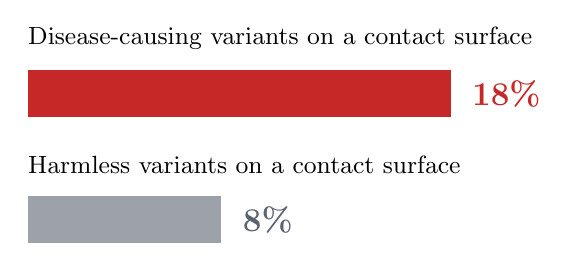
\begin{tikzpicture}[x=3mm]
        \node[anchor=west,font=\small,inner sep=0pt] at (0,23mm) {Disease-causing variants on a contact surface};
        \fill[patho] (0,13mm) rectangle (17.9,19mm);
        \node[anchor=west,font=\large\bfseries,text=patho] at (18.4,16mm) {18\%};
        \node[anchor=west,font=\small,inner sep=0pt] at (0,7mm) {Harmless variants on a contact surface};
        \fill[mute!60] (0,-3mm) rectangle (8.2,3mm);
        \node[anchor=west,font=\large\bfseries,text=mute] at (8.7,0mm) {8\%};
      \end{tikzpicture}

      \vspace{3mm}
      {\scriptsize\color{mute}2,260 of 12,655 pathogenic and 677 of 8,247 benign
      ClinVar missense variants, in 906 proteins that have both.\par}
    \end{column}
    \begin{column}{0.42\textwidth}
      \points{
        \item Compared fairly, protein by protein, the odds are \textbf{2.4×}
          (between 2.0 and 2.8)
        \item It is not just ``the mutation is in a solid part of the protein'':
          on the folded surface alone it is \textbf{3.2×}
        \item So a contact surface is a reason to look harder at a variant
          nobody has classified yet
      }
    \end{column}
  \end{columns}
\end{frame}

\begin{frame}
  \frametitle{TL;DR: on the team's receptors, AlphaFold's predicted contact surfaces match the lab's}
  \framesubtitle{Using team dataset 1}
  \begin{columns}[T,onlytextwidth]
    \begin{column}{0.55\textwidth}
      \shot[trim=0 300 0 0]{\textwidth}{gpcr.png}
    \end{column}
    \begin{column}{0.42\textwidth}
      \points{
        \item 45 lab-solved receptor structures picked by the team; 23 include
          the G protein the receptor signals through
        \item Where both exist, the predicted surface covers
          \textbf{87–90\%} of the experimental one
        \item \textbf{10 known disease mutations} sit where the Gs
          protein docks to receptors; AlphaFold DB has no prediction there
      }
    \end{column}
  \end{columns}
\end{frame}

\begin{frame}
  \frametitle{TL;DR: one gene makes several versions of a protein, and some versions lose a contact surface}
  \framesubtitle{Gene versions (isoforms)}
  \begin{columns}[T,onlytextwidth]
    \begin{column}{0.4\textwidth}
      \points{
        \item We lined up 7,648 alternative versions against the standard one
        \item \textbf{290} lose half or more of a contact surface
        \item \textbf{2,123} lack a position where a disease mutation is known
        \item Example: the brain's version of APP, the Alzheimer's protein,
          lacks the part that binds three protease partners
      }
    \end{column}
    \begin{column}{0.57\textwidth}
      \shot[trim=0 300 0 0]{\textwidth}{isoforms_APP.png}
    \end{column}
  \end{columns}
\end{frame}

\begin{frame}
  \frametitle{TL;DR: these are leads, not proof, and there is room to take it further}
  \framesubtitle{Honest limits and next steps}
  \begin{columns}[T,onlytextwidth]
    \begin{column}{0.47\textwidth}
      {\small\bfseries Limits\par}\vspace{1.5mm}
      \points{
        \item Most contact surfaces are AI predictions, not measurements
        \item Only 1 in 4 disease proteins has a predicted partner
        \item A variant on a contact surface is a hint about how it does harm,
          not a diagnosis
      }
    \end{column}
    \begin{column}{0.47\textwidth}
      {\small\bfseries Open for the team\par}\vspace{1.5mm}
      \points{
        \item Which of the 23,233 unclassified variants deserve a closer look?
        \item The 22 receptor structures without a G protein are not analysed
          yet
        \item The contact-surface lists are plain JSON and bigBed files: could
          Mol*, iCn3D or Jalview show them too?
      }
    \end{column}
  \end{columns}
\end{frame}

\appendix

\begin{frame}
  \frametitle{Pathogenic variants sit at predicted interfaces 2.4× as often as benign ones}
  \framesubtitle{Backup · the statistics}
  \lede{\footnotesize Within-protein comparison (Mantel–Haenszel odds ratio, bootstrap 95\%
  CI) over the 906 proteins with both pathogenic and benign missense variants.}
  \begin{columns}[T,onlytextwidth]
    \begin{column}{0.6\textwidth}
      \begin{tikzpicture}[y=-5.2mm]
        \foreach \t in {2,3,4}
          \draw[rule,line width=0.4pt] ({\orx{\t}},1.5) -- ({\orx{\t}},8.6);
        \draw[mute,dashed,line width=0.4pt] ({\orx{1}},1.5) -- ({\orx{1}},8.6);
        \foreach \t in {1,2,3,4}
          \node[font=\tiny,text=mute] at ({\orx{\t}},9.1) {\t};
        \node[font=\tiny,text=mute] at ({\orx{2.5}},9.9) {Odds ratio (1 = no difference)};
        \node[anchor=west,font=\tiny\bfseries,text=mute,fill=paper,inner sep=1pt] at (-31mm,1) {WHICH RESIDUES ARE COMPARED (ipSAE ≥ 0.6)};
        \forest{2}{All residues}{2.39}{2.01}{2.82}
        \forest{3}{Folded (pLDDT ≥ 70)}{1.70}{1.44}{2.01}
        \forest[patho]{4}{Folded, surface-exposed}{3.24}{2.66}{3.95}
        \node[anchor=west,font=\tiny\bfseries,text=mute,fill=paper,inner sep=1pt] at (-31mm,5) {CONFIDENCE THRESHOLD (ALL RESIDUES)};
        \forest{5.9}{ipSAE ≥ 0.6}{2.39}{2.01}{2.82}
        \forest{6.7}{ipSAE ≥ 0.7}{2.38}{2.00}{2.81}
        \forest{7.5}{ipSAE ≥ 0.8}{2.03}{1.61}{2.58}
        \forest{8.3}{ipSAE ≥ 0.9}{1.81}{0.94}{3.98}
      \end{tikzpicture}
    \end{column}
    \begin{column}{0.38\textwidth}
      \smallpoints{
        \item It is \textbf{not just ``folded vs disordered''}: among folded,
          surface-exposed residues the odds ratio is 3.2 (2.7–4.0)
        \item The signal \textbf{does not strengthen with confidence}: flat
          near 2.4 up to ipSAE 0.7, then lower, with far fewer variants left at
          the stricter thresholds
      }
    \end{column}
  \end{columns}
\end{frame}

\begin{frame}
  \frametitle{From a gene to its partners and its interface variants}
  \framesubtitle{Backup · gene pages}
  \begin{columns}[T,onlytextwidth]
    \begin{column}{0.61\textwidth}
      \shot[trim=0 120 0 0]{\textwidth}{gene_GNAO1.png}
    \end{column}
    \begin{column}{0.36\textwidth}
      \smallpoints{
        \item \textbf{GNAO1:} pathogenic variants at the Gβ interface (L13P,
          I19M, L23F) and the RGS interface (T182I, Q205P, R206)
        \item \textbf{VHL:} 48 pathogenic variants at the elongin C interface
        \item The 23,233 variants of uncertain significance at an interface
          are the leads
        \item Tracks carry one feature per partner, e.g. ``GNAO1–GNB2 (ipSAE
          0.73)''
      }
    \end{column}
  \end{columns}
\end{frame}

\begin{frame}
  \frametitle{Reproducible, tested, and deployed on every push}
  \framesubtitle{Backup · engineering}
  \vspace{2mm}
  \begin{columns}[T,onlytextwidth]
    \begin{column}{0.5\textwidth}
      \footnotesize
      \begin{tabular}{@{}l>{\raggedright\arraybackslash}p{44mm}@{}}
        \toprule
        \textbf{When} & \textbf{Milestone} \\
        \midrule
        10 Nov & Prototype: AlphaFold DB interfaces and ClinVar on hg38; website around JBrowse \\[1mm]
        11 Nov, am & Every disease gene; ClinVar from NCBI; isoform browser \\[1mm]
        11 Nov, pm & Isoforms for all 3,423 genes; GPCR page from the team's selection, with chimeric Gα \\[1mm]
        11 Nov, eve & Pipeline ported from Python to TypeScript; type check and tests gate the deploy \\
        \bottomrule
      \end{tabular}
    \end{column}
    \begin{column}{0.46\textwidth}
      \smallpoints{
        \item \textbf{Seven pipeline steps} in TypeScript, run directly by
          Node 24 with no build step: \texttt{pnpm all}
        \item Built on \textbf{g2p\_mapper} and \textbf{p2s\_mapper}, the
          libraries behind the JBrowse protein3d plugin
        \item The port reproduces the Python outputs: all four BED files byte
          for byte
        \item \textbf{79 unit tests} in 12 files
        \item GitHub Actions deploys the static site with JBrowse Web to Pages
      }
    \end{column}
  \end{columns}
\end{frame}

\end{document}
